
\documentclass[10pt]{beamer}

\usepackage{graphicx}
\usepackage{xcolor}
\usepackage{amsfonts}
\usepackage{amsmath}
\usepackage{amssymb}
\usepackage{centernot}
\usepackage[skip=10pt plus1pt] {parskip}

%Information to be included in the title page:
\title{Numbers \& Objects}
\author{UChicago Political Science Math Camp}
\institute{Ryan Gibbons \& Luke Cain}
\date{2025}

\begin{document}

\frame{\titlepage}

\begin{frame}{What is a set?}
    A set is a collection of elements. (That's it.)
\pause

    A set may consist of numbers, qualitative elements, or anything in between, and is contained by curly brackets. \\

    \[\{1,2,3\}\]
    \[\{\text{UChicago, Northwestern, Loyola, UIC}\}\]
    \[\{\text{Luke}, \pi, \theta, \text{Ryan}, 8\}\]
\pause

    A set can even consist of other sets, or of nothing at all.

    \[\emptyset\]

\end{frame}

\begin{frame}{Sets in Political Science}
    \begin{itemize}
        \item All countries (by some given definition)
        \item All countries recognized by China
        \item Legislators on a committee
        \item Voters in a society
        \item Possible GDP values
        \item Possible GDP-per-capita values
    \end{itemize}
\end{frame}

\begin{frame}{Properties of Sets}
    \begin{itemize}
        \item A set is not defined by its order:
        \[\{1,2,3\} \equiv \{3,2,1\}\]

        \pause
        \item A set has a \textbf{cardinality}, the number of its elements, represented by $\#$ or $|\{ \}|$:
        \[\#\{A,B,C\} = |\{1,2,3\}| =  3\]
        \pause

        \item A set with a cardinality of 1 is called a \textbf{singleton.}
        \pause

        \item We can use cardinality to determine \textbf{finite} versus \textbf{infinite} sets:
        \[\#\{1,2\} = 2\]
        \[\#\{\text{All numbers between 1 and 2}\} = \infty\]
    \end{itemize}
\end{frame}


\begin{frame}{The Empty Set}
    We define the \textbf{empty set}, a set containing no elements, as $\emptyset$. \\
\vspace{1cm}
Examples include:
\begin{itemize}
    \item The set of all autocracies with free and fair elections
    \item Former Soviet states in Africa
    \item Senators representing the District of Columbia
\end{itemize}

\end{frame}

\begin{frame}{Set Operations}
    We can (and often do) work with \textbf{set operations}, which return certain elements in some range of sets. \\

    \vspace{.5cm}

    Let 

    \[A = \{1,2,3,4,5\} \quad \quad B = \{1,3,5,7,9\} \]\\
\vspace{2cm}
    \begin{footnotesize}
        \textit{@Ryan write this on the board}
    \end{footnotesize}
\end{frame}

\begin{frame}{Union}
    The \textbf{union} of $A$ and $B$ is written as $A \cup B$ and defines all elements in \textit{either} $A$ or $B$.

    \begin{center}
        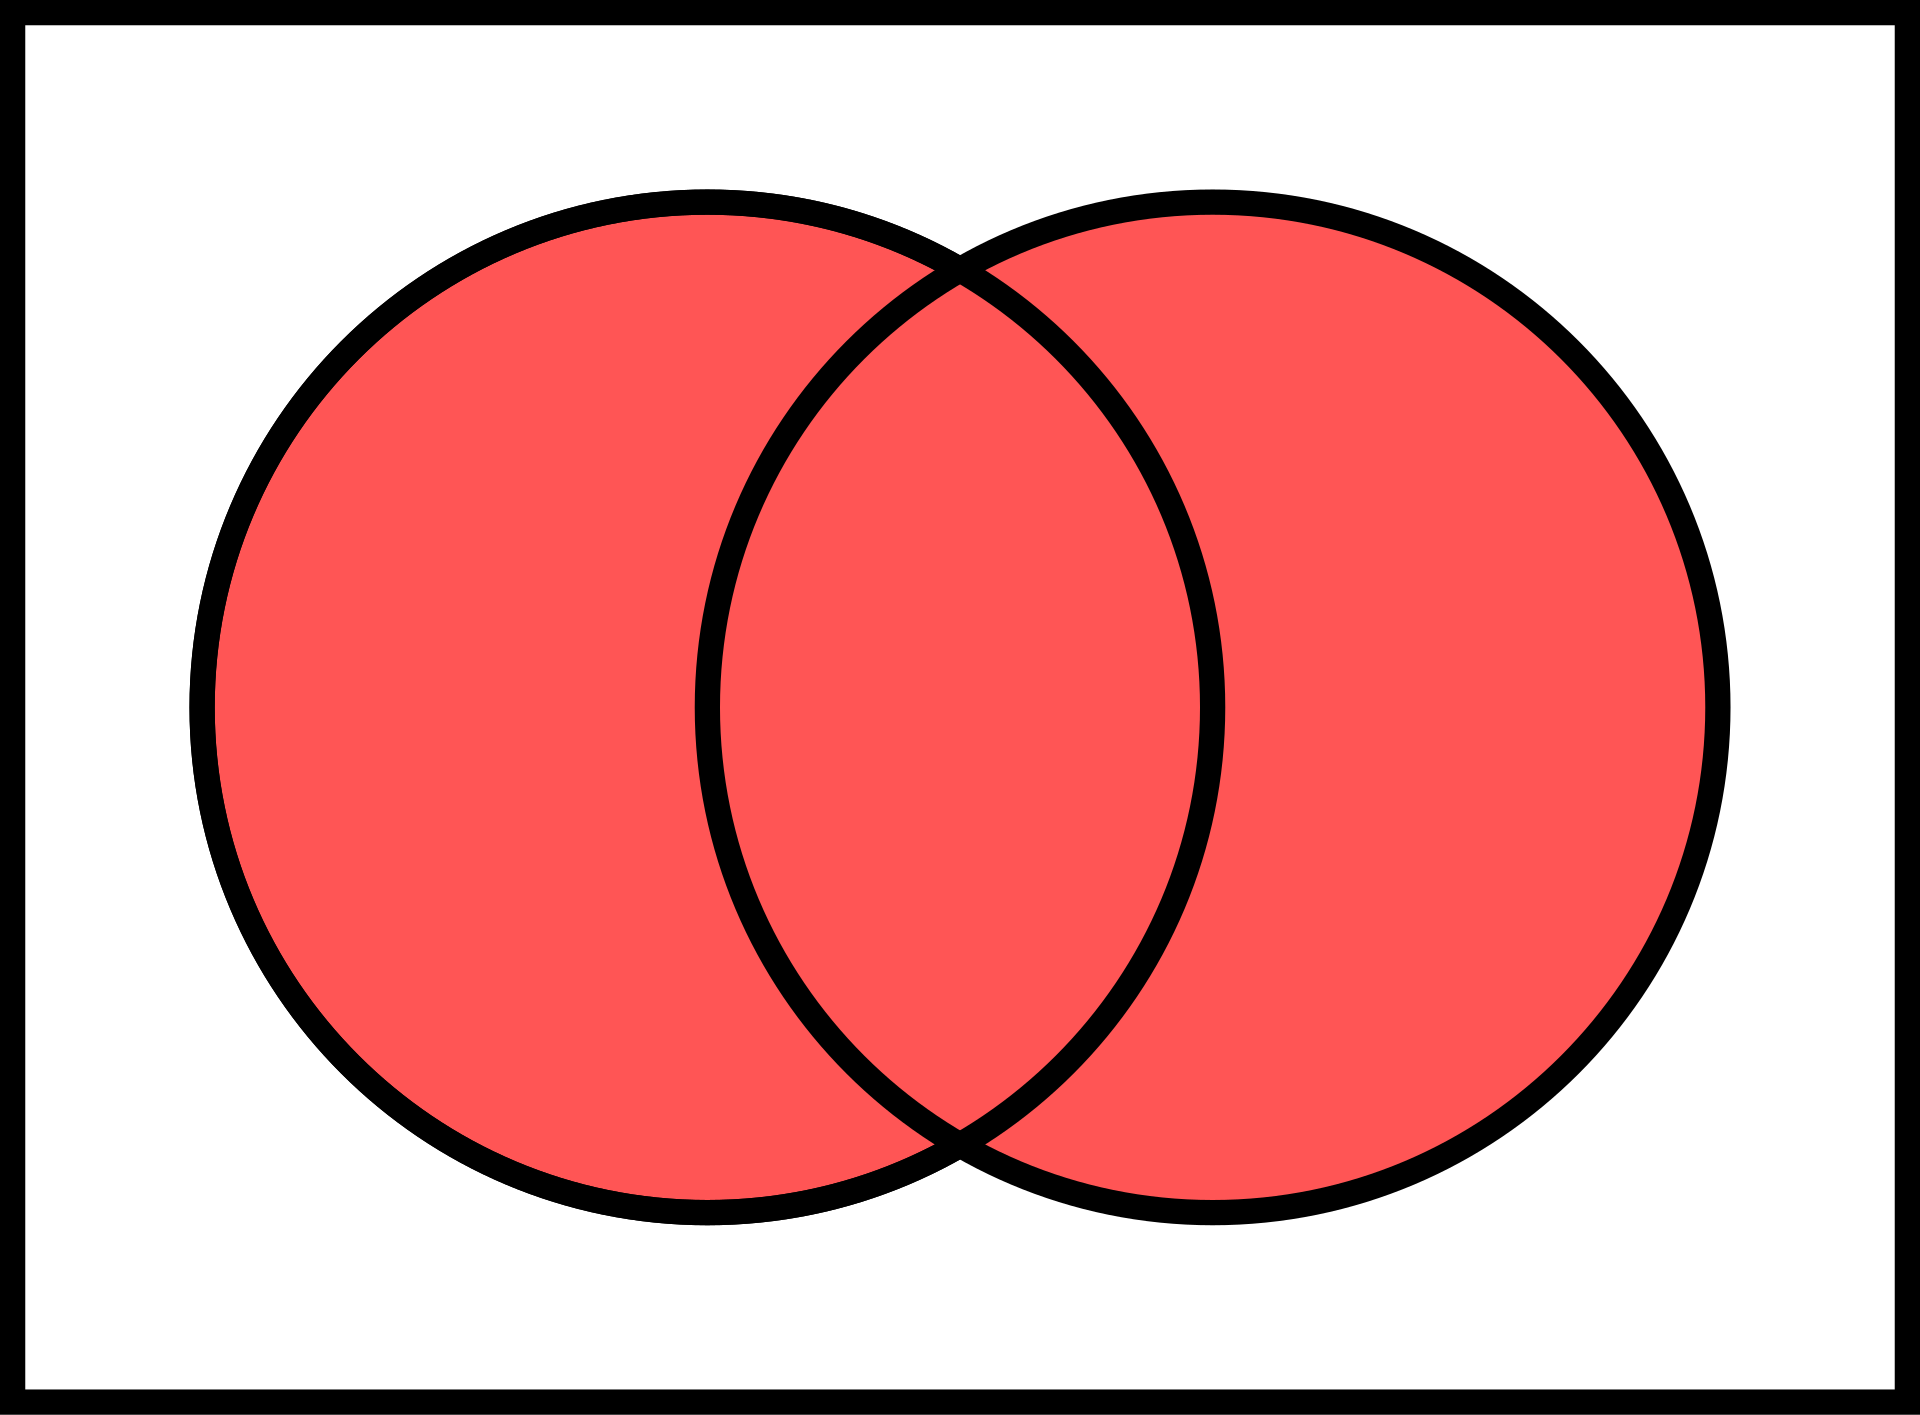
\includegraphics[width=5cm]{union.png}
    \end{center}

    What is $A \cup B$? \\

    \pause

    \[A \cup B = \{1,2,3,4,5,7,9\}\]
\end{frame}

\begin{frame}{Intersection}
    The \textbf{Intersection} of $A$ and $B$ is written as $A \cap B$ and defines all elements in \textit{both} $A$ and $B$.

    \begin{center}
        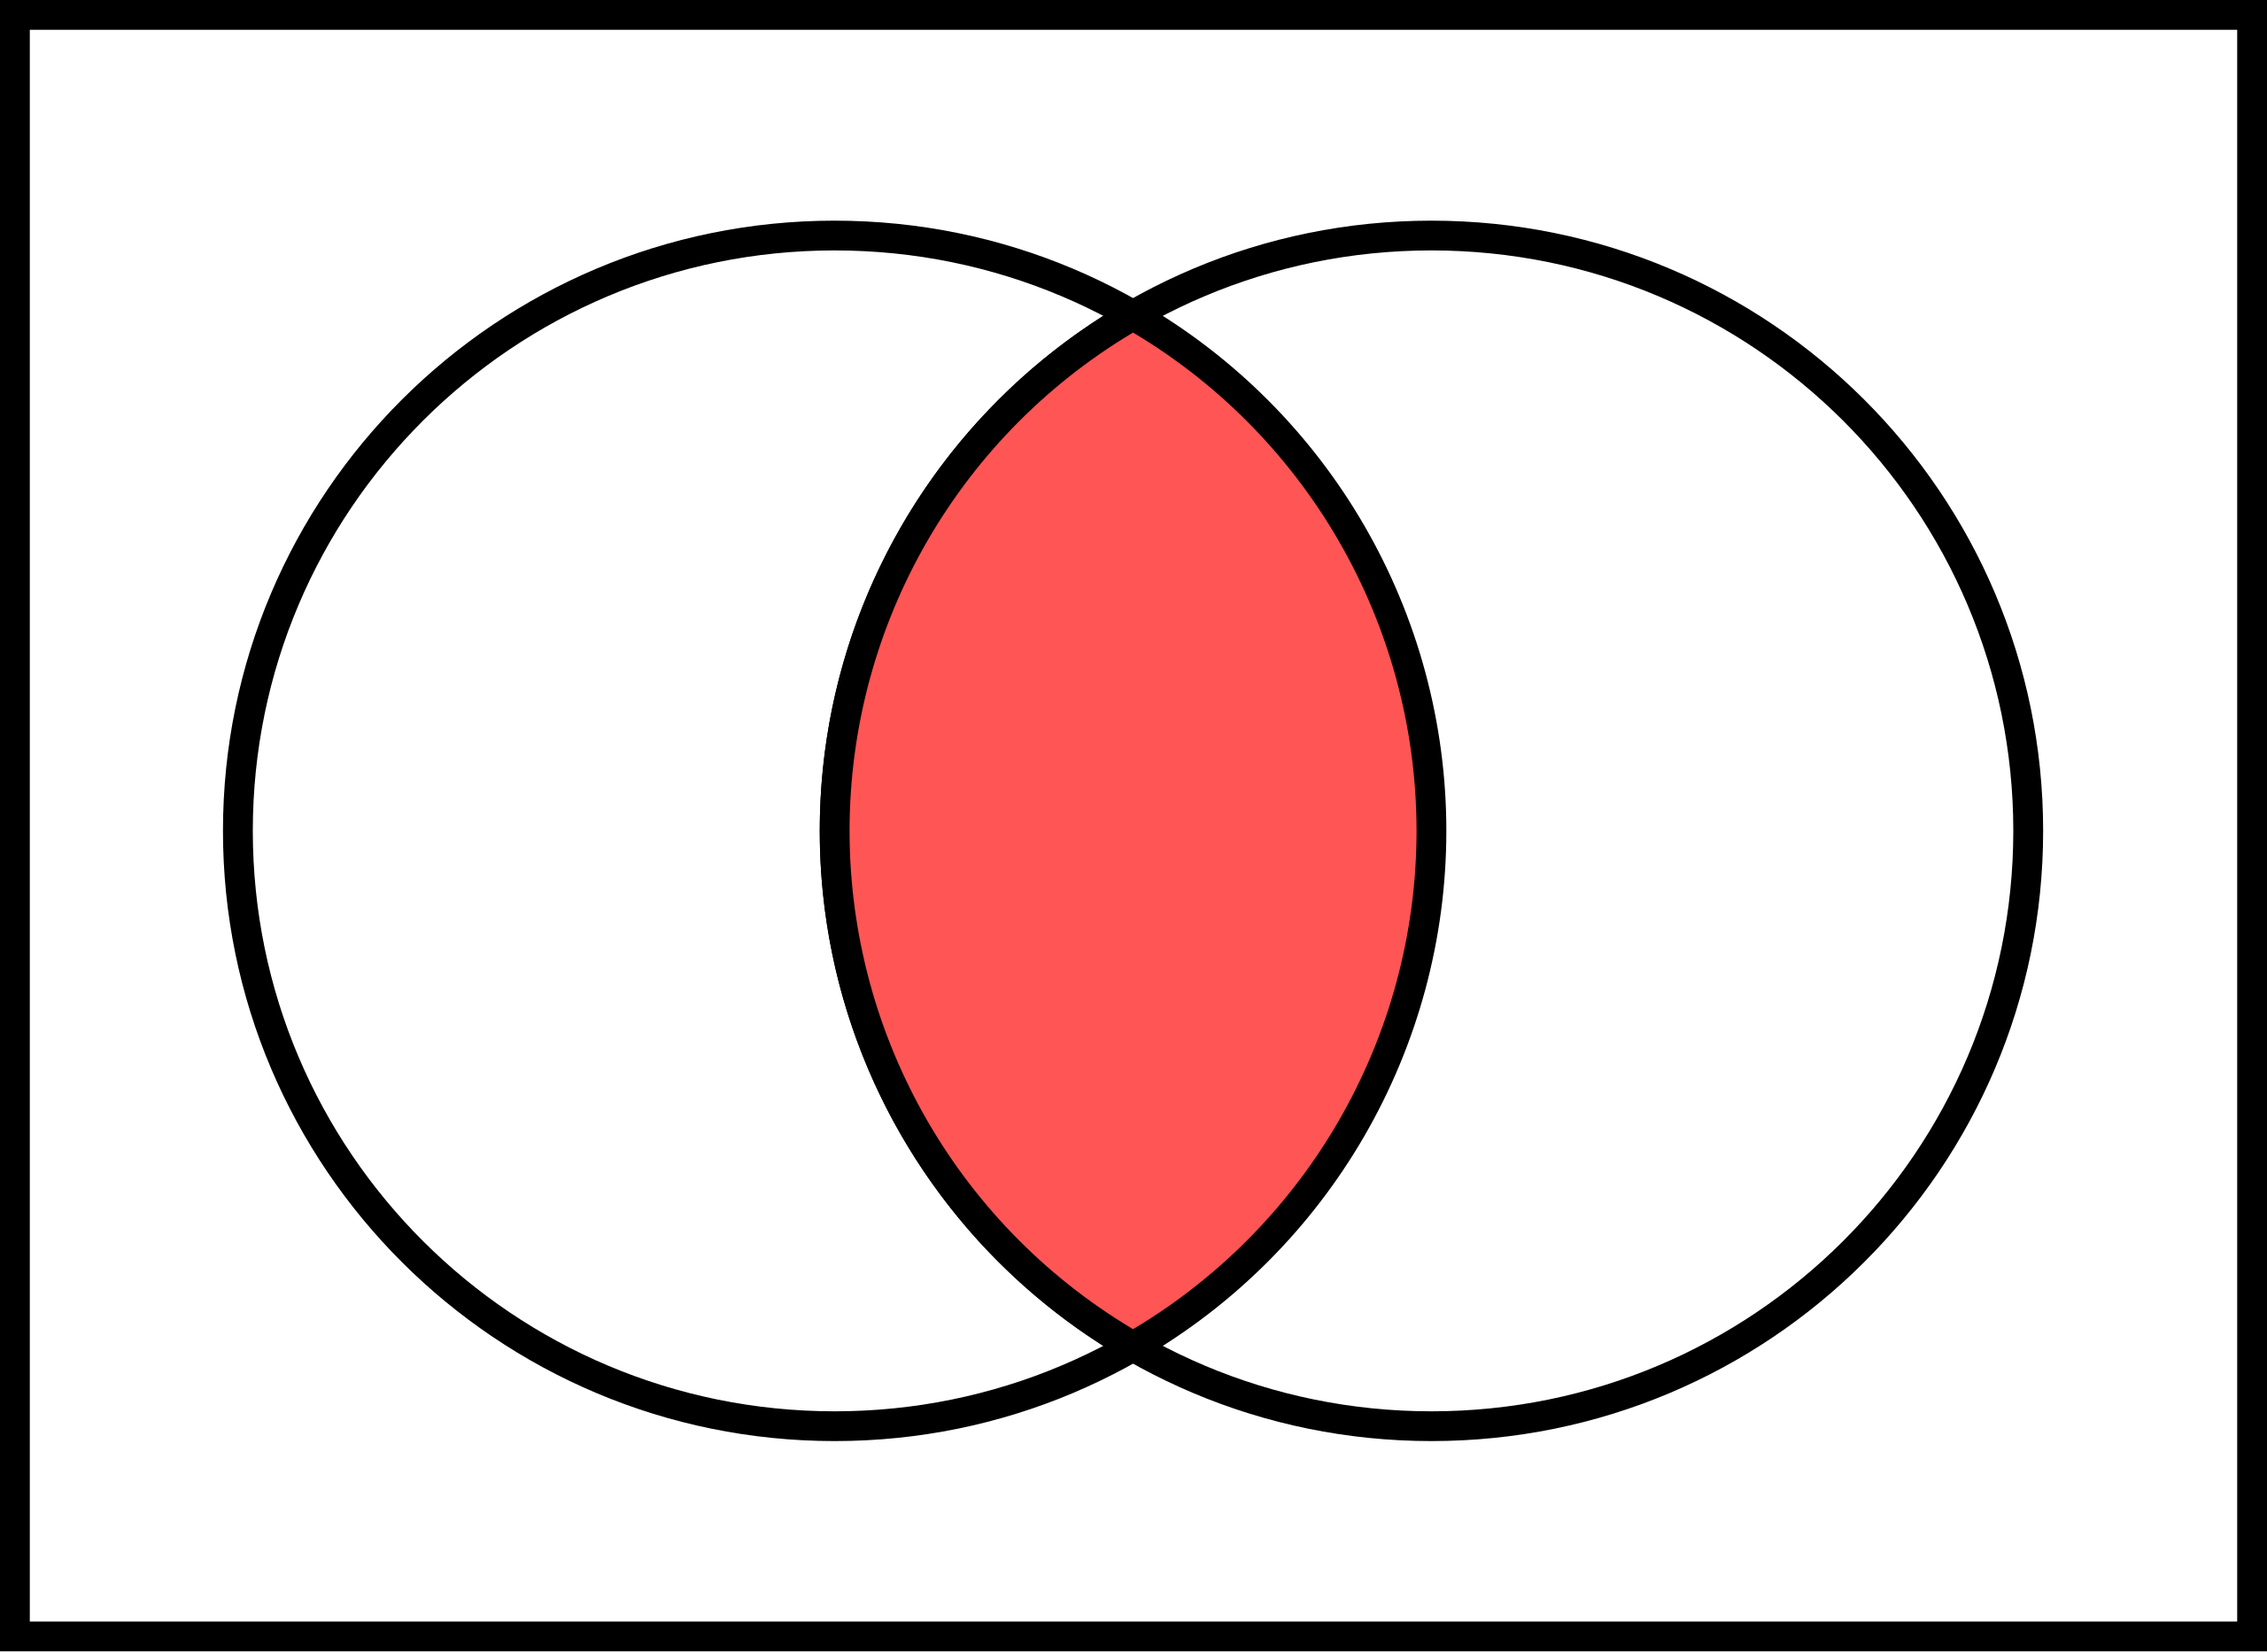
\includegraphics[width=5cm]{intersection.png}
    \end{center}

    What is $A \cap B$? \\

    \pause

    \[A \cap B = \{1,3,5\}\]
\end{frame}

\begin{frame}{Sample Space \& Complement}
    The \textbf{sample space} is all of the possible outcomes being considered. (Sometimes called the \textbf{universe}) \\
    \vspace{.5cm}
    The \textbf{complement} of a set $A$ is written as $A^C$ and defines every element of the sample space that is \textit{not} in an element of $A$. \\

    \begin{center}
        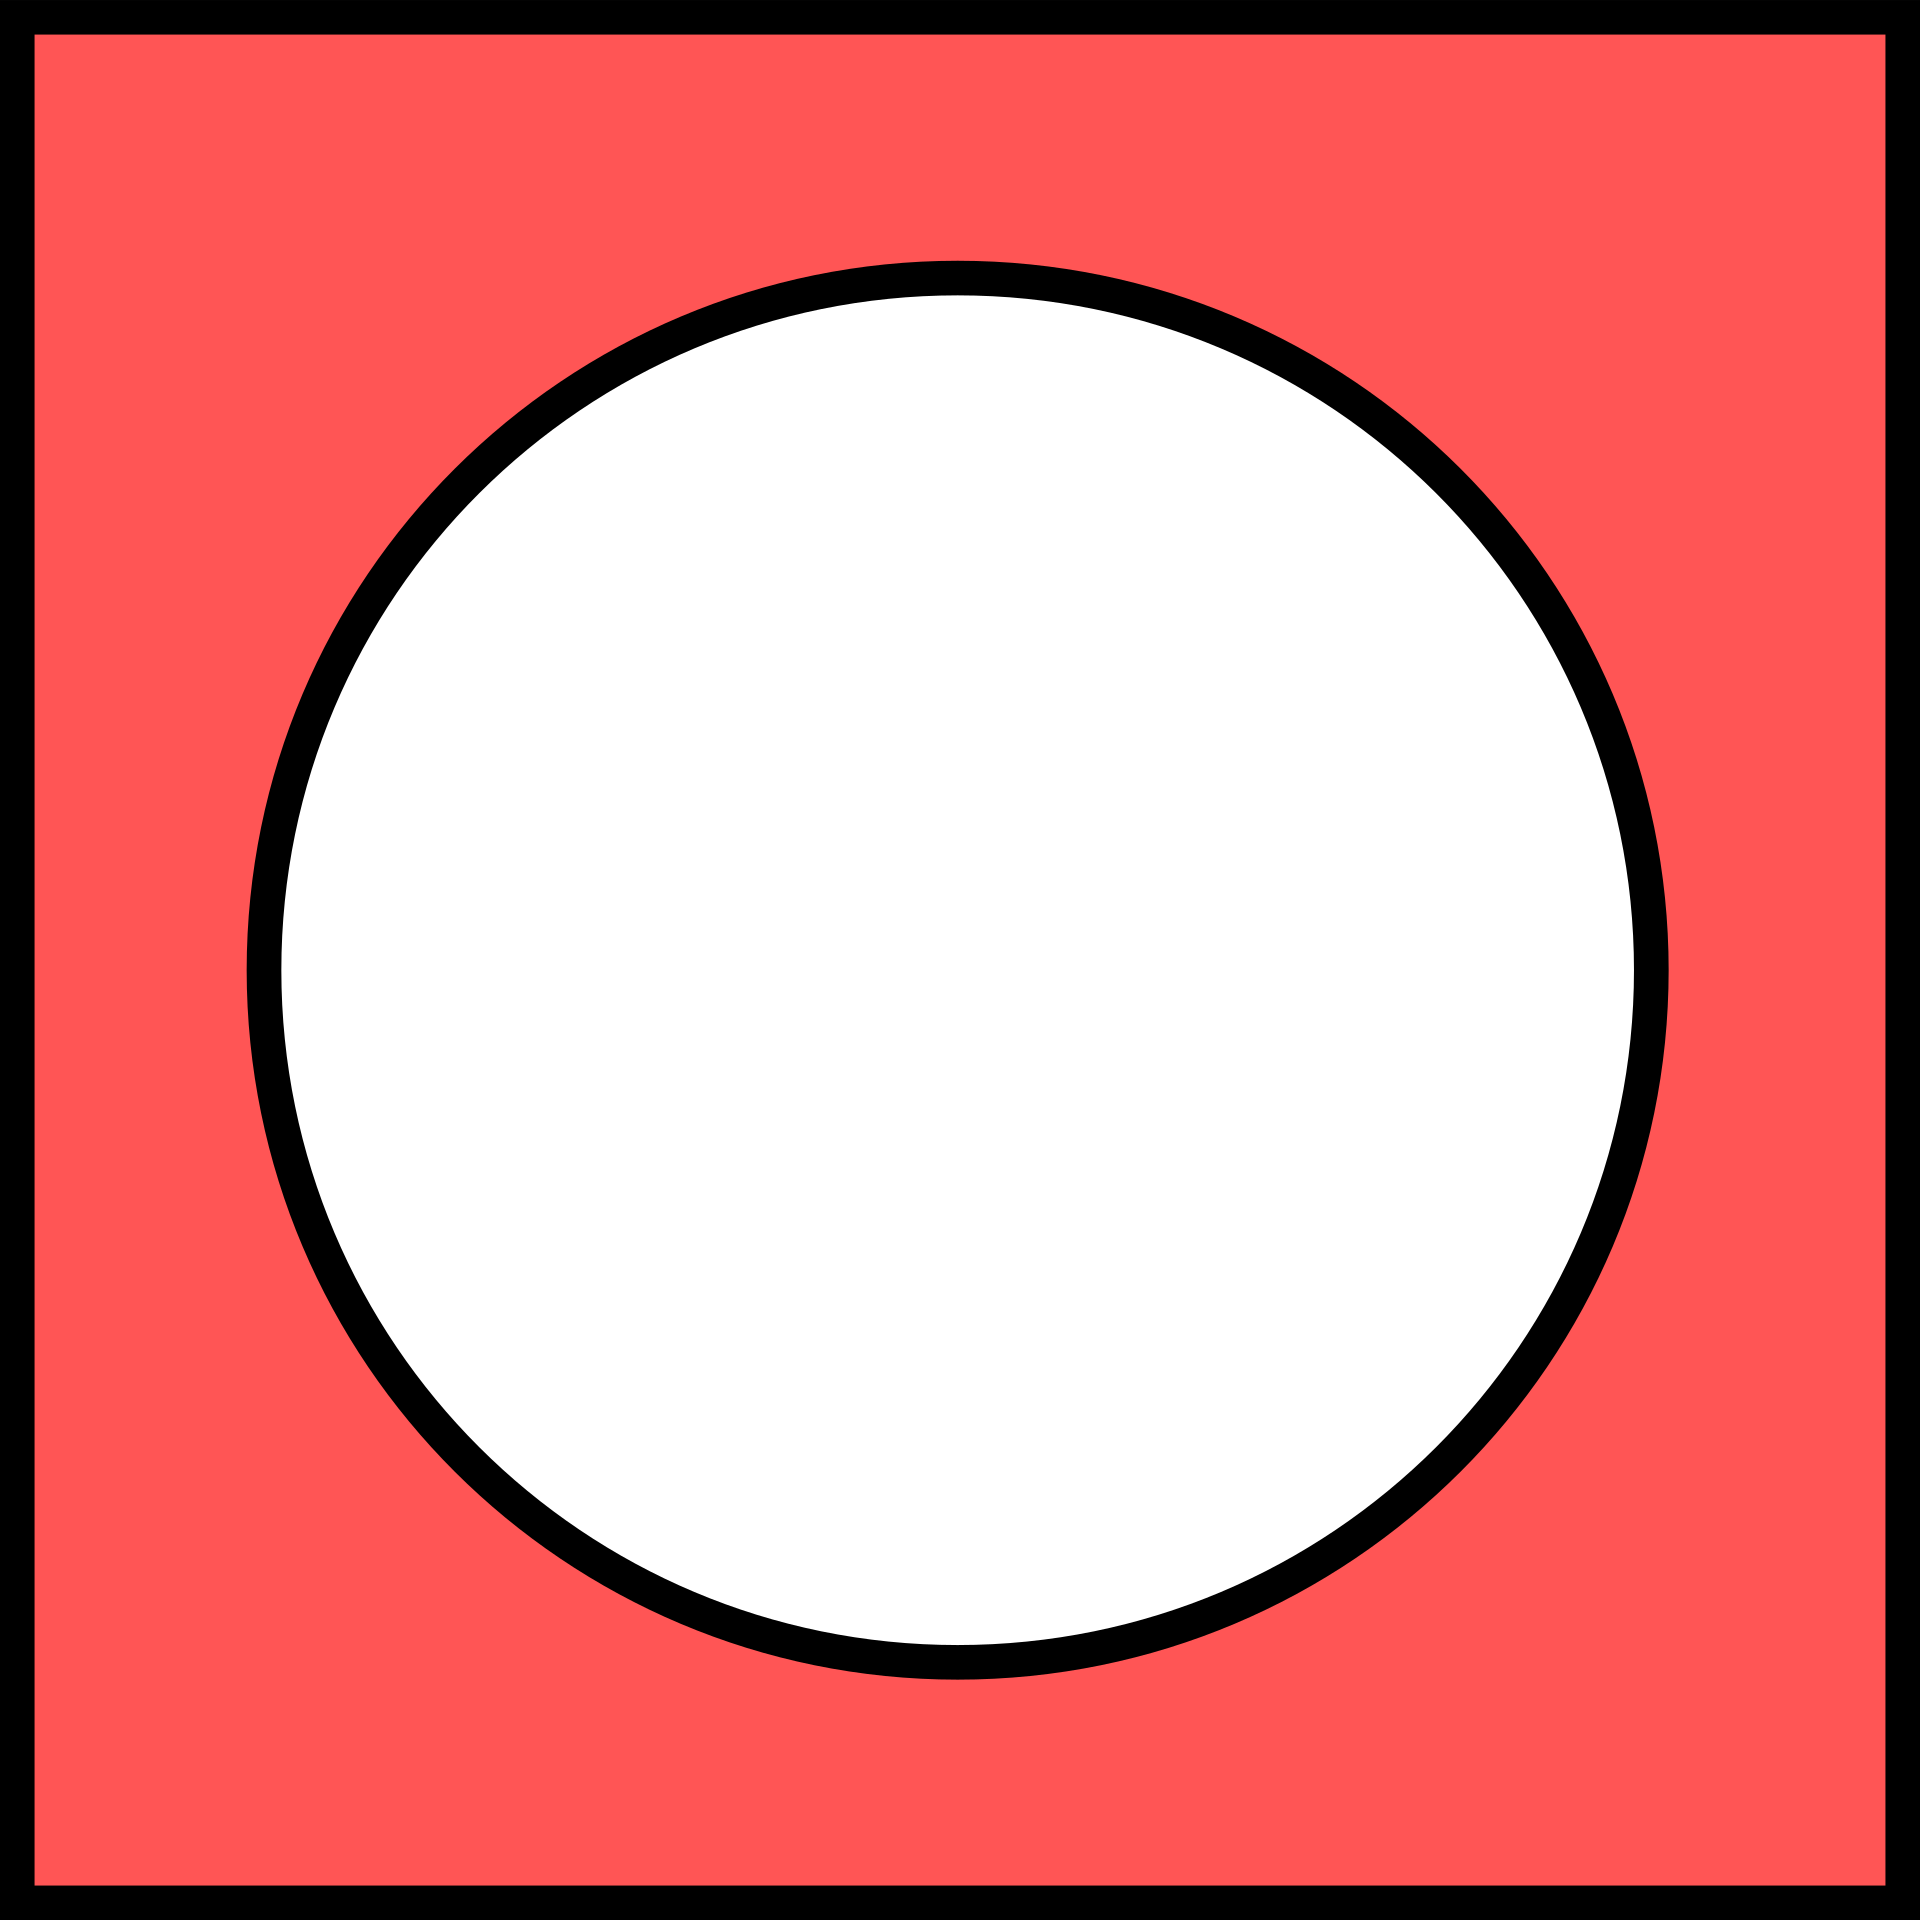
\includegraphics[width=5cm]{complement.png}
    \end{center}

\end{frame}

\begin{frame}{Complement Examples}
    Let the sample space be defined as $S = \{1,2,...,10\}$. Define the following:

    \begin{itemize}
        \item $A^C$ \pause
        \item $B^C$ \pause
        \item $(A \cup B)^C$ \pause
        \item $(A \cap B)^C$ 
    \end{itemize}
\end{frame}

\begin{frame}{Symmetric Difference}
    The \textbf{Symmetric Difference} of $A$ and $B$ is written as $A \Delta B$ and defines all elements in \textit{either} $A$ and $B$, but \textit{not} in \textit{both} $A$ and $B$.

    \begin{center}
        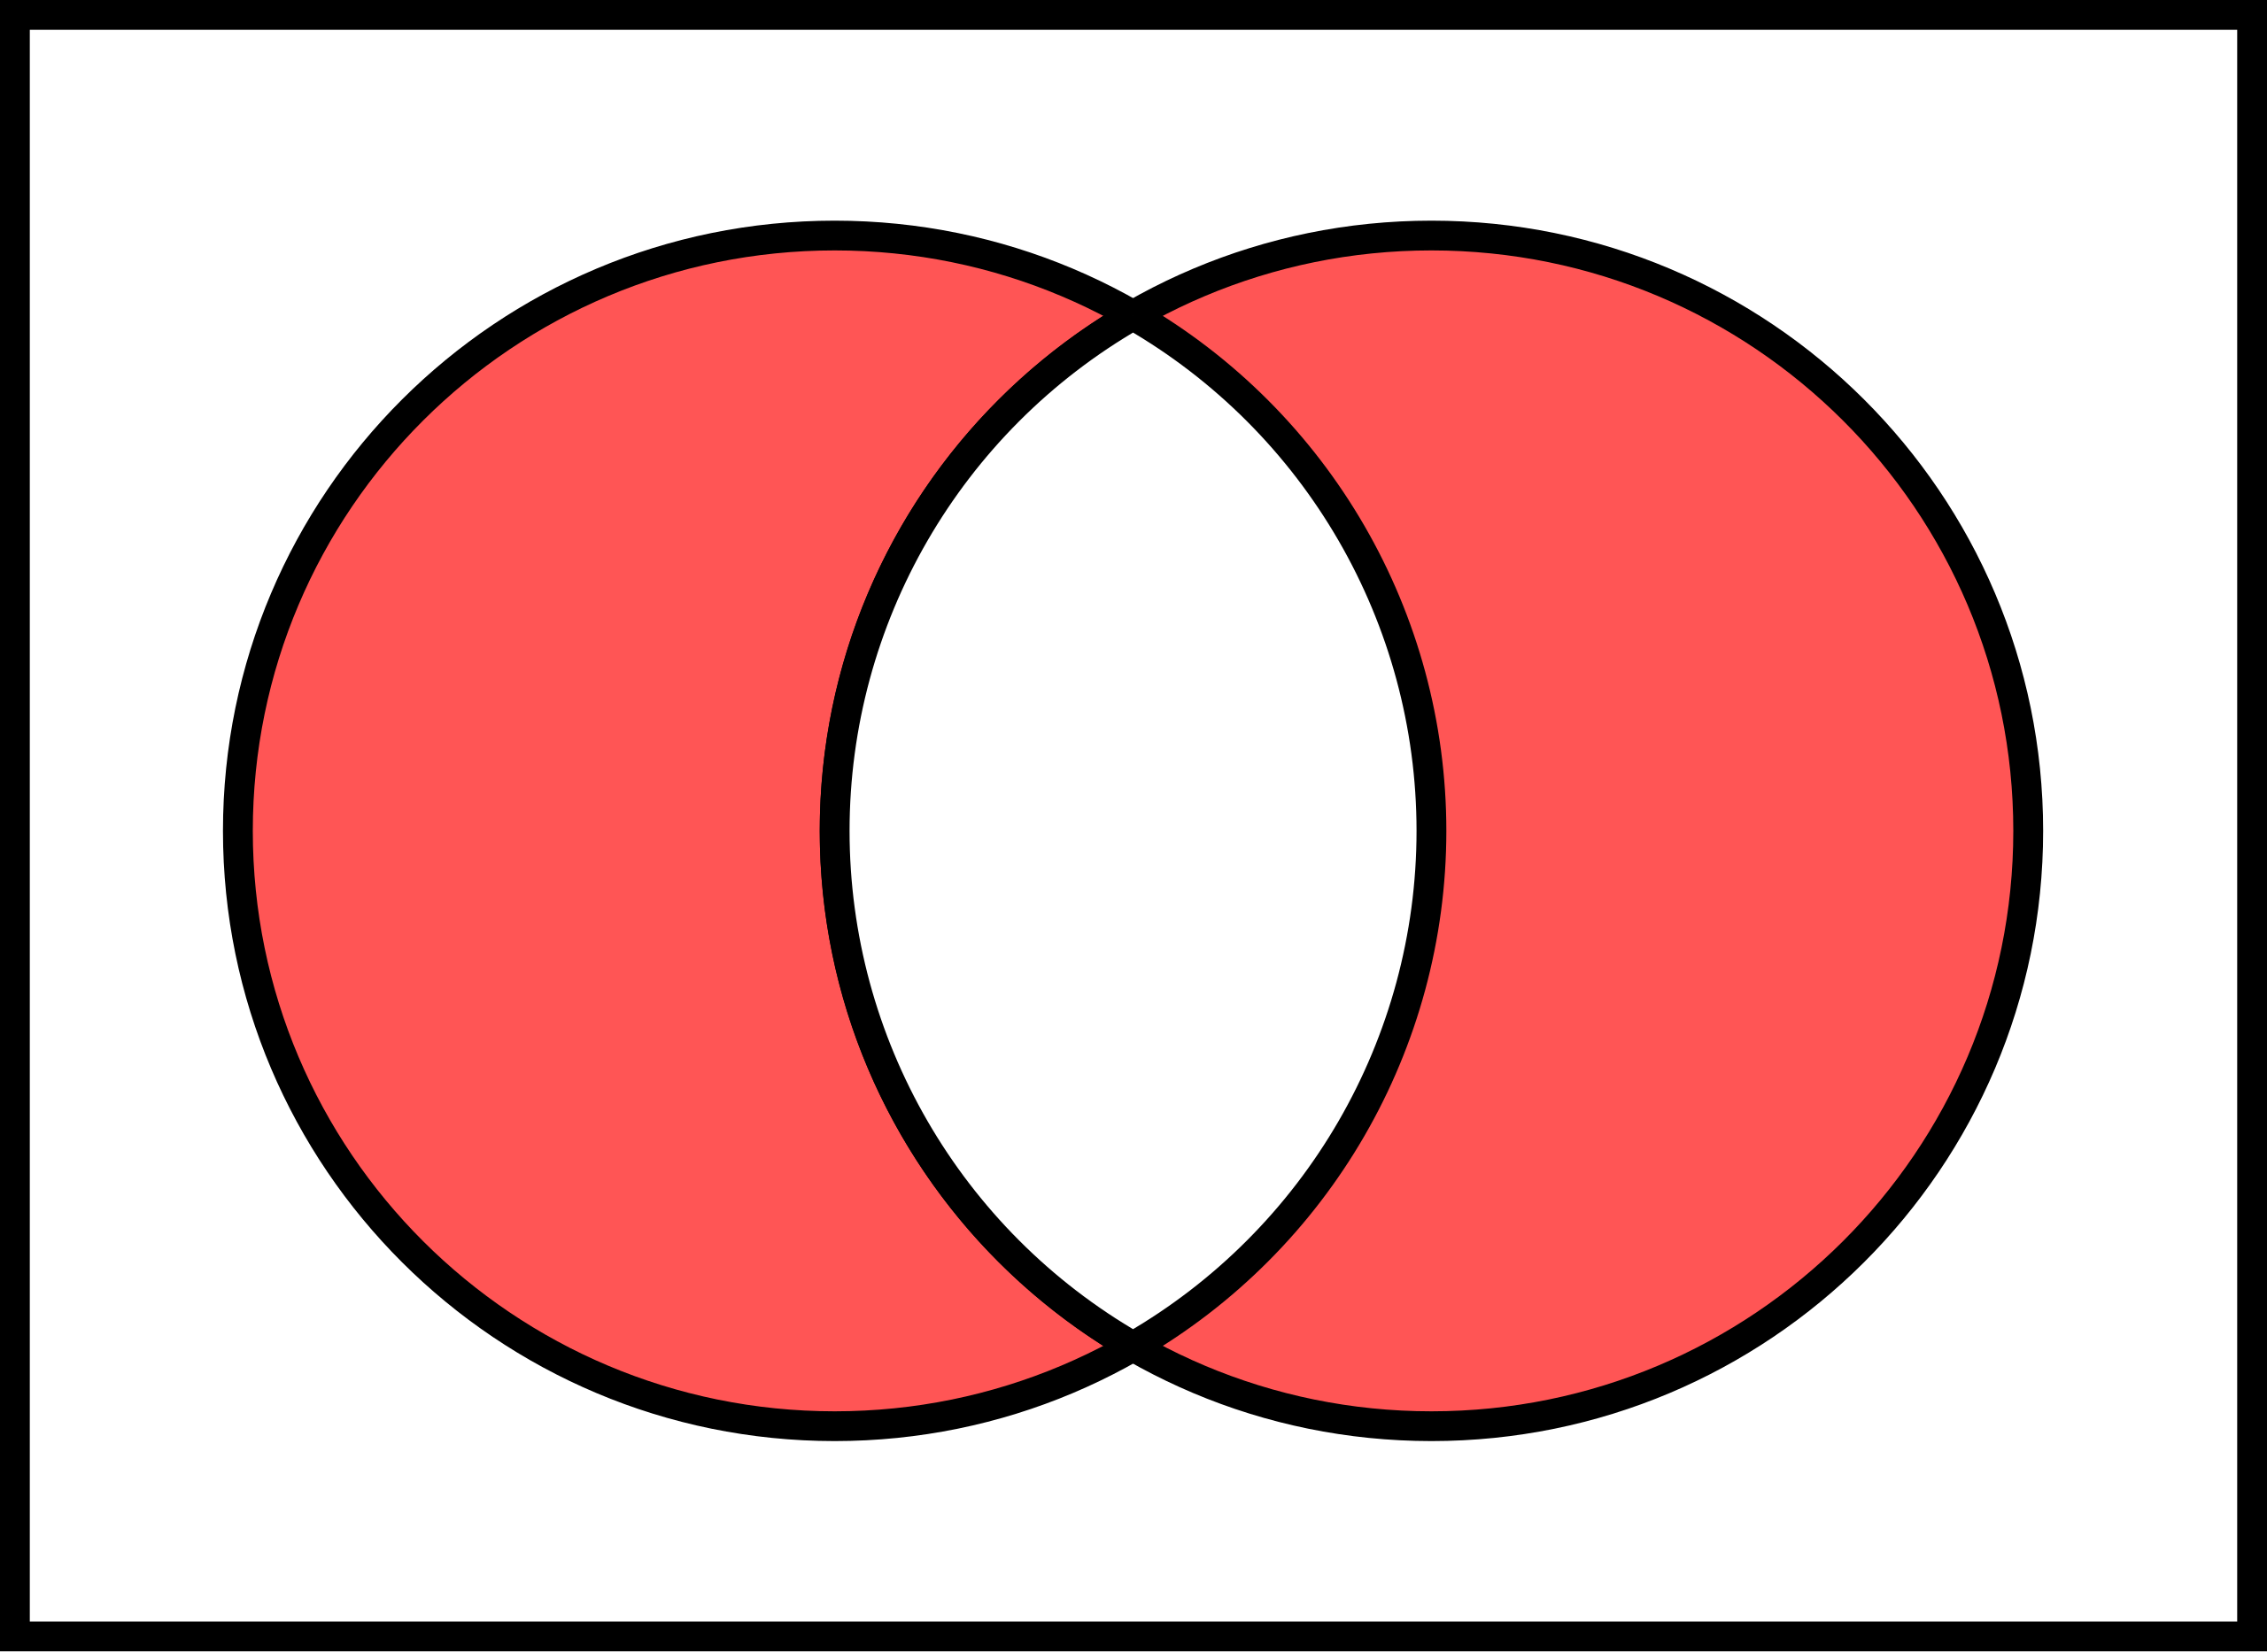
\includegraphics[width=5cm]{symmetricdifference.png}
    \end{center}

    What is $A \Delta B$? \\

    \pause

    \[A \Delta B = \{2,4,7,9\}\]
\end{frame}

\begin{frame}{Set Operations}
    Let us define $S = C$ as the set of counting numbers from 1 to 10, and

    \[A = \{1,2,3,4,5\} \quad \quad B = \{1,3,5,7,9\} \]

    \begin{itemize}
        \item Union: 
        \[A \cup B  ? \quad \quad B \cup C  ?\]
        \item Intersection:
        \[A \cap B ? \quad \quad B \cap C ?\]
        \item What if $D = \{2,4,6,8,10\}$? $B \cup D?$ $B \cap D$?
    \end{itemize}
\end{frame}

\begin{frame}{Set Operations}


    \begin{itemize}
        \item Excluding:

        \[A \setminus B ? \quad \quad C\setminus B ?\]
        
        \item Complement:

        \[A^C  ? \quad \quad B^C  ?\]

        \item Symmetric Difference:

        \[A \Delta B ? \quad \quad B \Delta C = ?\]
    \end{itemize}
\end{frame}

\begin{frame}[fragile]{Back To Elements}
    We use the symbol $\in$ to represent \verb|\in|:
    \begin{align*}
        x \in A \implies x \text{ is an element of }A
    \end{align*}

    Similarly, we use $\notin$ to represent \verb|\notin|:
    \begin{align*}
        x \notin A \implies x \text{ is not an element of }A
    \end{align*}
\end{frame}

\begin{frame}{Subsets}
    Some set $m$ is a \textbf{subset} of set $n$ if every element in $m$ is also an element in $n$.

    \[A \subseteq C\]

    Some set $m$ is a \textbf{proper subset} of $n$ if every element in $m$ is also an element in $n$ \underline{and} there exists some element in $n$ that is not in $m$.

    \[A \subset C\]

    This implies:
    \begin{align*}
        C &\subseteq C \\
        C &\not\subset C
    \end{align*}
\end{frame}

\begin{frame}{Reframing the Condition}
    We can use the definition of a subset to create a logical ``test'': 

    \textcolor{gray}{\textit{$M$ is a \textbf{subset} of set $N$ if every element in $M$ is also an element in $N$.}} \\
    $\implies$ \textcolor{red}{If every element in $M$ is also an element in $N$}, then $M \subseteq N$.

    Formally, 
    \begin{align*}
        (x \in M \implies x \in N) & \implies M \subseteq N
    \end{align*}
    \pause

    What about proper subsets?
    \begin{align*}
        \Big((x \in M \implies x \in N) \text{ and } (y \in N \centernot\implies y \in M)\Big) \implies M \subset N
    \end{align*}
\end{frame}

\begin{frame}{A Preview to Formal Logic}
    We often want to categorize conditions as \textbf{necessary}, \textbf{sufficient}, or both/neither:
\begin{itemize}
    \item A condition is \textbf{necessary} for an outcome if it MUST be met in order for the outcome to be true.
    \item A condition is \textbf{sufficient} for an outcome if its being met REQUIRES that the outcome is true.
\end{itemize}

\textit{Question: Which is stronger?}
\end{frame}

\begin{frame}{Tying Back}
    Consider the following condition:

    \textit{Every element of $m$ is also an element of $n$}


    Is this condition necessary and/or sufficient for the following outcomes?
\begin{enumerate}
    \item $m \subset n$
    \item $m \subseteq n$
\end{enumerate}
\vspace{.7cm}
\pause
\textcolor{red}{An important conclusion: $m \subset n$ implies $m \subseteq n$, but $m \subseteq n$ does not imply $m \subset n$. \emph{``Proper Subset'' is a \underline{stronger} condition.}}
\end{frame}

\begin{frame}{Power Sets}
    The \textbf{power set} is the set of all subsets of a set (phew).

    Let $n = \{A,B\}$. Then,

    \[P^n = \Big\{ \{A,B\},\{A\},\{B\},\{\emptyset\}\Big\}\]

    Let $m = \{A,B,C\}$. Then,

    
        \begin{align*}
        P^m = \Big\{&\{A,B,C\},\{A,B\},\{B,C\},\{A,C\},\\ 
        &\{A\},\{B\},\{C\},\{\emptyset\}\Big\}
        \end{align*}
    

    Note that $\#[P^X] = 2^{\#[X]}$.
\end{frame}

\begin{frame}{Your turn:}


$A = \{4,5,6\}$ \\
$B = \{5,6,7\}$.

Identify the following and explain what each refers to:

\begin{itemize}
    \item $A \cup B$

    \item $A \cap B$

    \item $B \setminus A$

    \item $A \Delta B$

    \item $\#P^B$
\end{itemize}

\end{frame}

\begin{frame}{Your turn:}


$A = \{51:59\}$ \\
$B = \{\text{Ellis, University, Woodlawn, Kimbark, Kenwood}\}$.

Identify the following and explain what each refers to:

\begin{itemize}
    \item $A \cup B$

    \item $A \cap B$

    \item $B \setminus A$

    \item $A \Delta B$

    \item $\#P^B$
\end{itemize}

\end{frame}

\begin{frame}{An Illustrating Example}
    \textit{The European Union / Eurozone / Schengen Area}
\end{frame}

\begin{frame}{A Step Back: Some Important Notation}

    We are learning a \textit{language} that is precise, but not necessarily unique. There are a few key symbols and phrases necessary to understand sets:

    \begin{itemize}
        \item $\in$ = ``in": $x \in A$ means $x$ is an element in $A$
        \pause
        \item $[a,b]$ = all elements from $a$ to $b$ (inclusive). (Occasionally expressed as $[a:b]$, especially in coding)
        \pause
        \item $(a,b)$ = all elements from $a$ to $B$ (exclusive)
        \pause
        \item $:$  read as ``such that" (sometimes just s.t.)
    \end{itemize}
\end{frame}

\begin{frame}{A Step Back: Set Builder Notation}

In order to fully understand the most important sets, we must understand how to write and read in \textbf{set-builder notation}. \\

A common format might look like this:

\[\text{name} = \{x \in \text{parent} \;: \; \text{condition 1, condition 2,...}\} \]

\begin{itemize}
    \item \underline{Set name} is usually a Phoenician or Greek letter
    \pause
    \item \underline{Parent} is what the set is being derived from - i.e., the real numbers (defined momentarily)
    \pause
    \item \underline{Conditions} are what defines the characteristics of the set.
    \pause
\end{itemize}

Let us go back to the zoo example:

\[\text{zoo mammals} = \{x \in \text{zoo animals} \; : \; \text{warm-blooded, vertebrate, has hair...} \}\]
\end{frame}

\begin{frame}{The Fundamental Sets}
    There are four fundamental sets in mathematics: $\mathbb{R}, \mathbb{N}, \mathbb{Z}, \mathbb{Q}$.

    Social scientists should understand $\mathbb{R}$ and $\mathbb{N}$.

    Quantitative social scientists should probably think about $\mathbb{Q}$ every once in a while.

    $\mathbb{Z}$ is extremely useful in applied mathematics, but doesn't come up much for us.
\end{frame}

\begin{frame}{The Real Numbers}
\begin{itemize}
\item Bulky definition, but: all well-defined numbers that can be placed on the number line \\

\item Expressed as $\mathbb{R}$ \\
\end{itemize}

The vast majority of political scientists only work with real numbers.
\end{frame}

\begin{frame}{The Natural Numbers}
    \begin{itemize}
        \item The ``counting numbers"

        \item Expressed as $\mathbb{N}$

    \end{itemize}
\textcolor{red}{Note that the natural numbers are strictly positive!}
\end{frame}

\begin{frame}{The Natural Numbers -- More Fun}
    But, why stop there?

    \[\mathbb{N} = \{x \in \mathbb{Z} \; : \; x + 1 > 1\}\]

    \[\mathbb{N} = \{x \in \mathbb{Z} \; : \; x \in [0,\infty)\}\]

    \[\mathbb{N} = \{x \in \mathbb{Z} \; : \; x \in \mathbb{R},\; x>0\}\]

    \[\mathbb{N} = \{x \in \mathbb{Z} \; : \; x \in \mathbb{R}_{++}\}\]

    \textit{There's usually many ways to write a set, and we want to choose the \textbf{simplest rigorous option.}}

\end{frame}

\begin{frame}{The Rational Numbers}
    \begin{itemize}
        \item All numbers that can be expressed as a fraction

        \item Formally:

        \[\mathbb{Q} = \{ x = \frac{a}{b} \; : \; a,b\in \mathbb{Z} , b \neq 0\}\]
\pause
        \item Note that 

        \[\mathbb{Q} \subset \mathbb{R}\]

        And since $1 \in \mathbb{Z}$,

        \[\mathbb{N} \subset \mathbb{Q}\]

        
    \end{itemize}
\end{frame}

\begin{frame}{The Integers}

\begin{itemize}
    \item The ``counting" numbers, both positive and negative

    \item Expressed as $\mathbb{Z}$, and defined as:

    \[\mathbb{Z} = \{x = a - b \;: \;a,b\in \mathbb{N} \}\]
\pause
    \item Note that $\mathbb{Z} \subseteq \mathbb{R}$, but NOT $\mathbb{R} \subseteq \mathbb{Z}$. Every natural number is real, but not all real numbers are natural.

    \begin{itemize}
        \item Note: this implies that $\mathbb{Z}$ is a proper subset of $\mathbb{R}$!
    \end{itemize}
\end{itemize}
\end{frame}

\begin{frame}{Above or Below $0$}
    Though we can use

    \[A = \{x \in \mathbb{R}:x \geq b \}\]

    to limit to only a specific subset, we are often most interested in the case where $b = 0$. Instead, we can express:

    \[\mathbb{R}_+, \mathbb{R}_-\]

    as shorthand for non-negatives ($\geq 0$) and non-positives ($\leq 0$), and

    \[\mathbb{R}_{++},\mathbb{R}_{--}\]

    as shorthand for positives ($>0$) and negatives ($<0$). Note that $\mathbb{N}_- = \emptyset$
\end{frame}

\begin{frame}{Your Turn:}
    Use set-builder notation to express each of the following in two different ways, making note of the simplest rigorous option:

    \begin{itemize}
        \item Example: All even numbers \\
        \pause
        \item Every number between $e$ and $\pi$
        \item All counting numbers less than $81$
        \item All integers that are the square root of another integer
        \item All real, irrational numbers
    \end{itemize}
\end{frame}



\begin{frame}{Defining Infinity}
    \begin{itemize}
        \item Each of the four primary sets $\mathbb{R,Z,N,Q}$ have infinite cardinalities.
        \item Every element of $\mathbb{Z,N,Q}$ can be mapped onto some value of $\mathbb{N}$, but \textit{not} every element of $\mathbb{R}$ (e.g. $\pi$)
        \item An infinite set for which each element can be mapped onto a natural number is \textbf{countably infinite}. Otherwise, it is \textbf{uncountably infinite}. 
    \end{itemize}
Note that  $\mathbb{Z,N,Q}$ all have the same cardinality (countable infinity), even though we can construct elements of $\mathbb{Z,Q}$ which are not elements of $\mathbb{N}$. Then, we need another definition....
\end{frame}



\begin{frame}{Closed vs. Open Sets}
    Not all infinite sets are created equally.

    Think: are $\mathbb{N}$ and $x \in \mathbb{R}: \{0 \leq x \leq 1\}$ similar in structure? 
    
    \pause
    
    What about $\mathbb{N}$ and $x \in \mathbb{R}: \{ 0 < x < 1\}$?

    \pause

    We can instead define an \textbf{open set} as one where no element is a clear boundary (and a \textbf{closed set} as its alternative).
\end{frame}


\begin{frame}{More Rigorously}
A set is open iff around every element of that set, you can always construct a \textbf{neighborhood} that is entirely within that set. 

That is, $A$ is an open set if, for every $x \in A$, there exists some set $B$ such that $x \in B$ and $B \subset A$. 
\end{frame}


\begin{frame}{Products of Sets}
    Oftentimes, we want to consider a set of all possible combinations of sets. We do so using the $\times$ operator:

    \begin{align*}
        \{1,2\} \times \{A,B\} &= \{(1,A),(1,B),(2,A),(2,B)\}
    \end{align*}

    When the sets are identical, we can just use exponents as shorthand
\end{frame}

\begin{frame}{Set Products \& Examples}
    In formal theory, we might often consider a ``state space.''

    A canonical example (largely driven by Açemoglu \& Robinson) considers the organization of the poor ($P$) and the elite ($E$) as either organized ($h$) or unorganized ($\ell$). The state space follows:

    \begin{align*}
        \Omega &= \{\text{Poor organization}\} \times \{\text{Elite organization}\} \\
        &= \{P^h, P^\ell\} \times \{E^h, E^\ell\} \\
        &= \{(P^h, E^h),(P^h,E^\ell),(P^\ell,E^h),(P^\ell,E^\ell)\}
    \end{align*}

    \emph{\textcolor{lightgray}{What are we encoding?}}
\end{frame}


\begin{frame}{Key Takeaways:}

\begin{itemize}
    \item Math is a \underline{language} -- precise, but not always consistent
    \item Focus on reading, not memorizing
    \item Let simplicity drive notation
\end{itemize}

\end{frame}


\end{document}